\section*{Anexo A. Resultados de Comparación de las Eficiencias de ICB}


Percentil-NVC

\begin{figure}[ht] 
	\centering 
	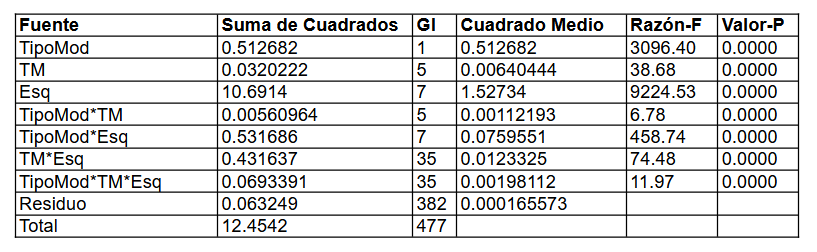
\includegraphics[width=0.95\linewidth]{img/ANOVA_Efic_ICB_Perc_NVC.png} 
	\caption{ANOVA para la eficiencia del ICB Percentil cuando se tiene NVC.} 
	\label{fig:ANOVA_Efic_ICB_Perc_NVC}
\end{figure}
\FloatBarrier



BCa-NVC

\begin{figure}[ht] 
	\centering 
	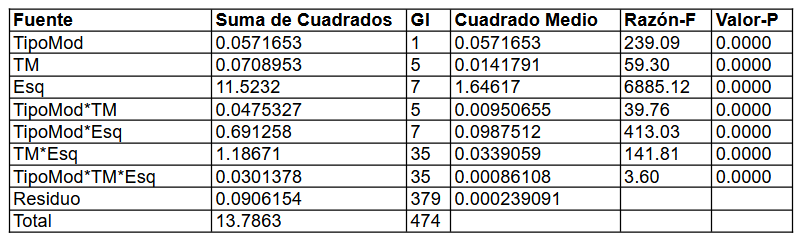
\includegraphics[width=0.95\linewidth]{img/ANOVA_Efic_ICB_BCa_NVC.png} 
	\caption{ANOVA para la eficiencia del ICB BCa cuando se tiene NVC.} 
	\label{fig:ANOVA_Efic_ICB_BCa_NVC}
\end{figure}
\FloatBarrier



%%%%%%%%%%%%%%%%%%%%%%%%%%%%%%%%%%%%%%%%%%%5

Percentil-NNVC

\begin{figure}[ht] 
	\centering 
	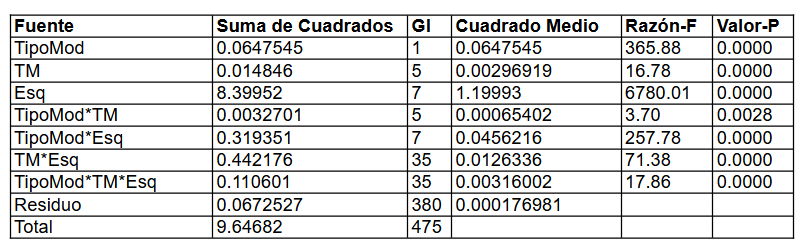
\includegraphics[width=0.95\linewidth]{img/ANOVA_Efic_ICB_Perc_NNVC.png} 
	\caption{ANOVA para la eficiencia del ICB Percentil cuando se tiene NNVC.} 
	\label{fig:ANOVA_Efic_ICB_Perc_NNVC}
\end{figure}
\FloatBarrier




BCa-NNVC

\begin{figure}[ht] 
	\centering 
	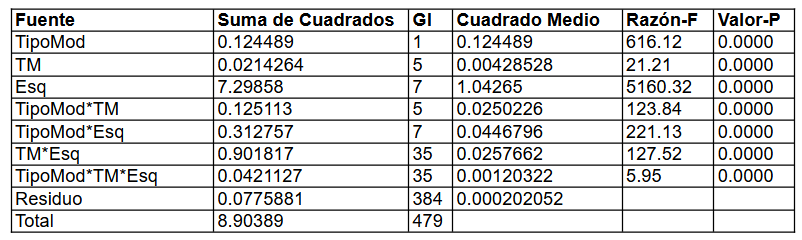
\includegraphics[width=0.95\linewidth]{img/ANOVA_Efic_ICB_BCa_NNVC.png} 
	\caption{ANOVA para la eficiencia del ICB BCa cuando se tiene NNVC.} 
	\label{fig:ANOVA_Efic_ICB_BCa_NNVC}
\end{figure}
\FloatBarrier





%%%%%%%%%%%%%%%%%%%%%%%%%%%%%%%%%%%%%%%%%%%5

Percentil-NVD

\begin{figure}[ht] 
	\centering 
	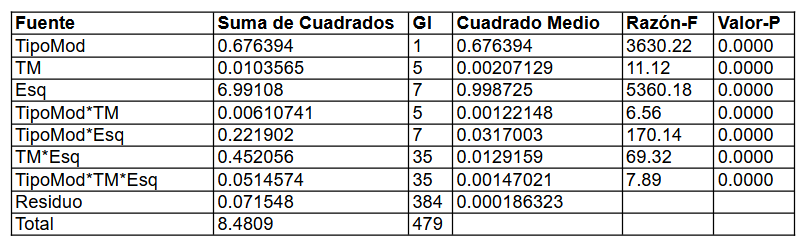
\includegraphics[width=0.95\linewidth]{img/ANOVA_Efic_ICB_Perc_NVD.png} 
	\caption{ANOVA para la eficiencia del ICB Percentil cuando se tiene NVD.} 
	\label{fig:ANOVA_Efic_ICB_Perc_NVD}
\end{figure}
\FloatBarrier






BCa-NVD

\begin{figure}[ht] 
	\centering 
	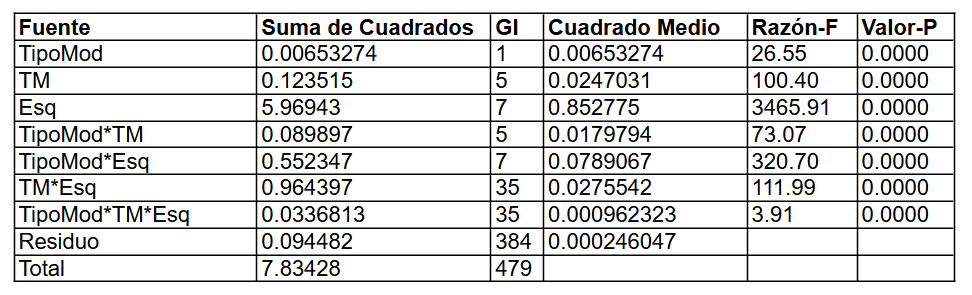
\includegraphics[width=0.95\linewidth]{img/ANOVA_Efic_ICB_BCa_NVD.png} 
	\caption{ANOVA para la eficiencia del ICB BCa cuando se tiene NVD.} 
	\label{fig:ANOVA_Efic_ICB_BCa_NVD}
\end{figure}
\FloatBarrier




%%%%%%%%%%%%%%%%%%%%%%%%%%%%%%%%%%%%%%%%%%%5

Percentil-NNVD

\begin{figure}[ht] 
	\centering 
	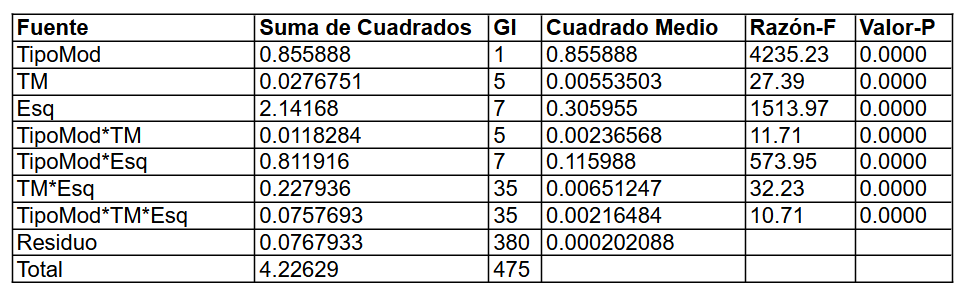
\includegraphics[width=0.95\linewidth]{img/ANOVA_Efic_ICB_Perc_NNVD.png} 
	\caption{ANOVA para la eficiencia del ICB Percentil cuando se tiene NNVD.} 
	\label{fig:ANOVA_Efic_ICB_Perc_NNVD}
\end{figure}
\FloatBarrier





BCa-NNVD

\begin{figure}[ht] 
	\centering 
	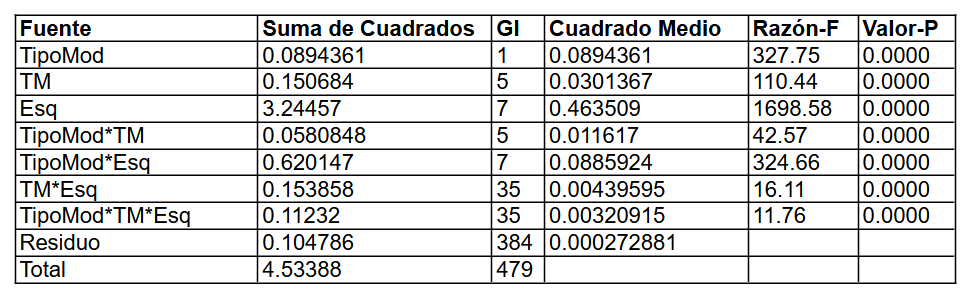
\includegraphics[width=0.95\linewidth]{img/ANOVA_Efic_ICB_BCa_NNVD.png} 
	\caption{ANOVA para la eficiencia del ICB BCa cuando se tiene NNVD.} 
	\label{fig:ANOVA_Efic_ICB_BCa_NNVD}
\end{figure}
\FloatBarrier


\newpage


\section*{Anexo A. Resultados de Comparación de las Eficiencias de ICB}






  